\section{Person Discovery challenge}
\label{sec:challenge}

Until very recently, research work relevant for the described task was dealing mainly with speaker or face recognition, with
few early attempts were both face and speaker identification tasks were treated simultaneously; the following review reflect
this situation.

For speaker identification, the closest modality for extracting the names of speakers was used: the pronounced names
from speech transcription. We can mention the works of Canseco et al. pioneered approaches relying on pronounced
names instead of biometric models for speaker identification [8] and [19]. They set manually linguistic patterns to
determine a link between a pronounced name and a speech segment. Following works improved this idea: [20] replaced
manual rules by learning sequence of n-grams with associated probabilities, [9], [21] and [14] used semantic classification
trees to calculate the probabilities, [22] replaced the decision by belief functions. However, due to relatively high speech
transcription and named entity detection errors, all these audio only approaches did not achieve good enough identification
performance.

Written names were first used for a face identification task in broadcast news ([23], [24]), but due to a high word error rate
(respectively 52 \% and 65 \%), these names were detected and corrected with the help of a dictionary (limiting identification
to a closed list of persons). Despite these corrections, the error rate was still very high (45 \% after correction in [24])
and consequently greatly limited the use of this source of information. Later, Yang et al. [25], [26] also tried to use
written names, but again, the video OCR system [27] used to process the overlaid text produced highly erroneous results
(e.g. “Newt Gingrich” was recognized as “nev j ginuhicij”). Their studies were limited to a single show (ABC World News
Tonight) and they only tries to label faces in monologue-style peech

We can also cite Pham et al. [28], [29], which first extracted a list of names from speech transcription. Then, they manually
associated a set of face images to these names. These identities are then propagated to the entire video from the similarity
between faces. They have therefore concentrated their works on the face identification and thus did not taken advantage
of the video multimodality with the use of speakers as indice for the propagation. Indeed, in [30] Khoury et al show that a
multimodal audio-visual diarization obtains better results than monomodal diarization.

Thanks to the REPERE challenge, significant progress was achieved in either supervised or unsupervised mulitmodal
person recognition. We proposed an unsupervised speaker/face identification system ([31], [32]) based only on written names
as source of names (extracted using the tool LOOV [10]) in TV broadcast. The main idea was to build mono-modal
clusters (faces or speakers) and to associate written names to these clusters based on their co-occurrences (un-supervised
approach). In this former work, faces and speakers were treated separately. This system was extended in [33], [34], [35], [36]
with the modification of the agglomerative clustering process.

This process integrated directly the knowledge of written names to both identify clusters and also to prevent the merging
of clusters named differently. We used this method during the presented campaign as the LIMSI system (Poignant et al. [37]
in Section V).

Another work that is worth being mentioned is using Integer Linear Programming (ILP) for speech clustering [38], [39],
[15]. The main idea is to replace the classical agglomerative BIC clustering by an ILP clustering and at the same time
integrating written names to identify speech clusters. First, multi-modal similarity graph is built, were intra-modal links
correspond to the similarity of mono-modal elements (speech turns: BIC distance, written names: identical or not) and crossmodal links correspond to the temporal co-occurrence between written names and speech turns. As a written name has a
high probability to match the current speaker, identification of speech turns via the ILP solver is equivalent to find the
less expensive way to connect names and speech turns. The main limitation of this method is the large computation time
for solving ILP (as well as the basic cross-modal link used).

In [40], speakers are named in the first place and then identities are propagated to visible persons. Speakers are named by
the propagation of written names and pronounced names and also with biometrics speaker models. After a face diarization
step, written names and speaker identities are propagated to faces based on their co-occurrence. Authors also integrate a
set of manual rules for a specific show to post-process their output (e.g. if one of the anchors is speaking and two faces
are detected, then the second face is given the identity of the second anchor). They extended these works in [41], [42] with
the use of automatic scene analysis (camera identification and scene classification as studio or report). This system needs
additional annotations (scene type, camera position) for a specific show. Once a camera has been identified, they can
deduct those who are visible on the screen (e.g., if the camera filming the anchor has been identified, they infer that the
anchor is visible in screen). Finally, [43] proposed to integrate a lip activity detector to propagate speakers identities to face.
Again, rules are used to propagate a name to a speaker/face. 

Last but not least, Gay et al. [44] proposed to propagate written names onto multi-modal speaker/face clusters. First,
speakers and face diarization are performed in parallel, then speaker and face clusters are grouped based on their cooccurrence. They are associated to written names with two methods. The first one relies on co-occurrence information between written names and speaker/face clusters, and rule-based decisions which assign a name to each mono-modal cluster. The second method uses a Conditional Random Field (CRF)
which combines different types of co-occurrence statistics and pair-wised constraints to jointly identify speakers and faces.

\mypartitle{Task overview.} Participants are provided with a collection of TV broadcast recordings pre-segmented into shots.
Each shot $s \in \shots$ has to be automatically tagged with the names of people both speaking and appearing at the same time during the shot: this tagging algorithm is denoted by $\hypLabels : \shots \mapsto \mathcal{P}(\hypNames)$ in the rest of the paper.

The list of persons is not provided \emph{a priori}, and person biometric models (neither voice nor face) can not be trained on external. The only way to identify a person is by finding their name $n \in \hypNames$ in the audio (\emph{e.g.} using ASR) or visual (\emph{e.g.} using OCR) streams and associating them to the correct person (Fig. \ref{fig:evidence}). %This makes the task completely unsupervised (\emph{i.e.} using algorithms not relying on pre-existing labels or biometric models). 
Because person names are detected and transcribed automatically, they may contain transcription errors to a certain extent (more on that later in Section~\ref{sec:metric}). In the following, we denote by $\refNames$ the set of all possible person names in the universe, correctly formatted as \texttt{firstname\_lastname} -- while $\hypNames$ is the set of hypothesized names.

\begin{figure}[!htb]
 \centering
 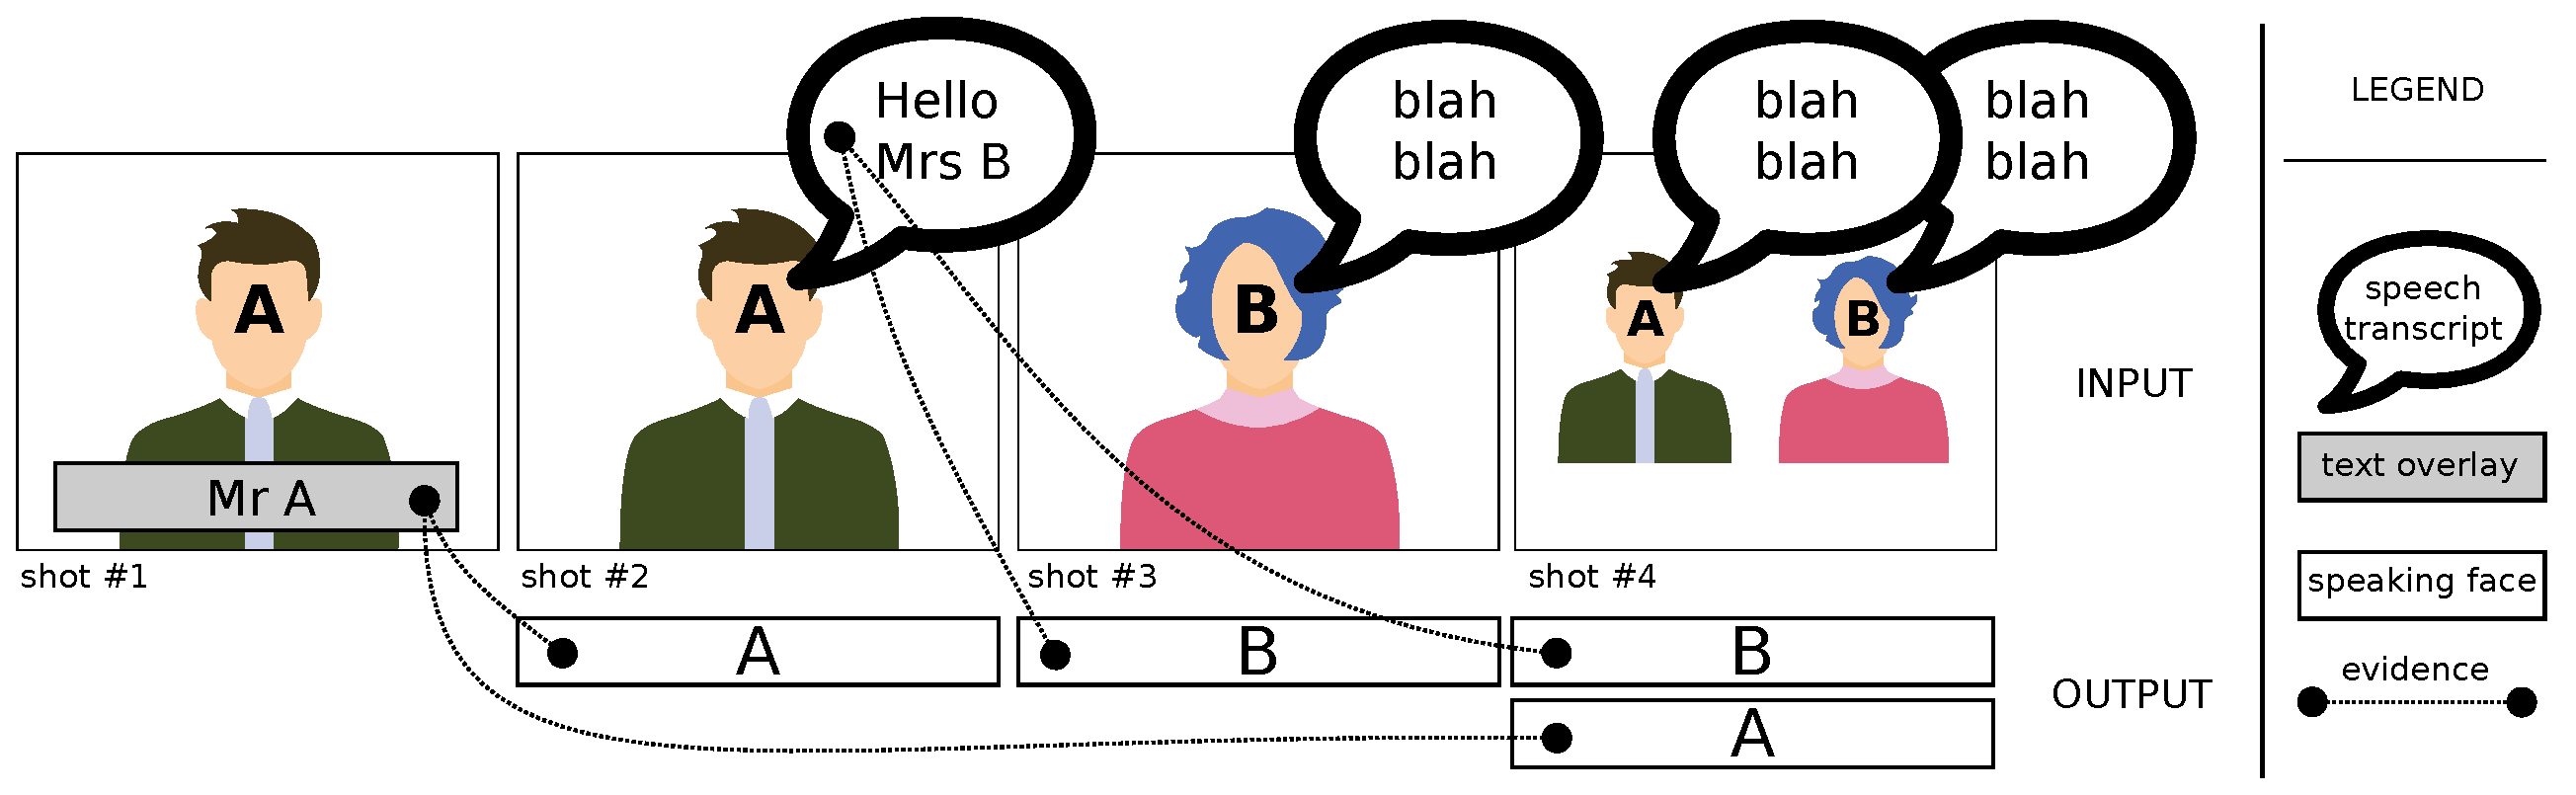
\includegraphics[width=1.\linewidth]{evidence.pdf}

 \caption{For each shot, participants have to return the names of every speaking face. An evidence is also returned for annotation process.}
 \label{fig:evidence}
\end{figure}

\mypartitle{Datasets and annotation.} The test set is divided into three datasets: INA, DW and 3-24. The INA dataset contains a full week of broadcast for 2 TV channels for a total duration of 90 hours in French. The DW dataset~\cite{EUMSSI} is composed of video downloaded from Deutsche Welle website, in English and German for a total duration of 50 hours. The last dataset contains 13 hours of broadcast from 3/24 Catalan TV news channel. Each shot has been tagged with the names of people who appear and speak within that shot.
%
\mycomment{Need more statistics on the dataset. Maybe a table should be sufficient.}

From the submissions of all participants, a set of hypotheses are generated for each shot. 
%
First thumbnail for a person. Correct names 
%
Second verify if that person 
%
Need statistics on the annotations (how many queries? shots? frequency of shots per name)

\mypartitle{Metrics.} The task is evaluated indirectly as an information retrieval task, using the folllwing principle.
%
For each query $q \in \queries \subset \refNames$ (\texttt{first\-name\_lastname}), returned shots are first sorted by the edit distance between the hypothesized person name and the query $q$ and then by confidence scores.
Average precision $\text{AP}(q)$ is then computed classically based on the list of relevant shots (according to the groundtruth) and the sorted list of shots. Finally, Mean Average Precision is computed as follows:
\begin{align}
            \text{MAP} & = \frac{1}{|\queries|} \sum_{q \in \queries} \text{AP}(q) \nonumber
\end{align}


\section{Overview of our approaches}
\label{sec:overview}

Basic of all approaches: people with similar faces and voices should have the same name. finding name candidates, propagates the names to similar appearances. Choke points: finding names, face / speech similarities, propagate names. Depends on how to deal with these choke points --> different approaches:

Overclusters ==> one name less, Underclusters ==> 1 less name. Tracking ==> build models based on names and propagated over other clusters. 

\mypartitle{Clustering-based naming.} 
Most common baseline. Face/speech tracks are first aggregated into homogeneous clusters according to person identities. Then each clusters is tagged with the most probable person name.

\mypartitle{Verification-based name propagation.} 
Clustering has 1 big disadvantage is relies on clustering. Error cannot be recovered. Higher priority on names, build discriminative models.
Verification.
A person name is first assigned to the most probable face/speech track. The name is then propagated to all face/speech tracks which are verified to have the same identity.

\mypartitle{Graph-based name propagation.} Another method to get around clustering. Verification is one-one, clustering is global. Graphbased more hybrid to make use of both.
A graph is built with a face/speech track as a node and weight of edges is the similarity. Some nodes are initially tagged with the names. Names are then propagated along the edges within the graph.

Clustering depends on models, verification and graphbased needs good names. Has different pros and cons, benchmarking to find best answers.
There are several problems related to these approaches such as face / speech representation, person diarization, or audio-visual verification. Each of these problems has been well studied within its respective context~\cite{recog,veri,rep}. 
%
However, these approaches have never been fully investigated and compared as whole systems in the large-scale multimedia indexing context before. In this paper, the authors aim to investigate all these approaches with variations in their components using real world datasets from TV news. 

discriminative, audio-visual combination, and minimize error rates.

The major drawbacks of clustering-based naming is its reliance on clustering results. 

\endinput